\documentclass{beamer}
\usetheme{Madrid}
\usecolortheme{default}
\usepackage{graphicx}
\usepackage{booktabs}

\title{Chef Classification with DistilBERT}
\author{NLP Group 2}
\institute{Instituto Superior Técnico}
\date{October 2025}

\begin{document}

\frame{\titlepage}

% Slide 1: The Task
\begin{frame}{The Task}
\begin{itemize}
    \item Predict which chef (out of 6) created a recipe
    \item \textbf{Data}: 2,999 training recipes, 823 test recipes
    \item \textbf{Features}: name, ingredients, tags, description, steps
\end{itemize}

\vspace{0.5cm}

\textbf{Baselines to beat}:
\begin{itemize}
    \item Weak (TF-IDF description only): 30\%
    \item Strong (TF-IDF all fields): 43\%
\end{itemize}
\end{frame}

% Slide 2: Approach
\begin{frame}{Our Approach}
\textbf{Model}: DistilBERT-base-uncased
\begin{itemize}
    \item 66M parameters (40\% smaller than BERT)
    \item Fine-tuned for 5 epochs
    \item Concatenate all text fields $\rightarrow$ classify
\end{itemize}

\vspace{0.5cm}

\textbf{Key decisions}:
\begin{itemize}
    \item Stratified train/val split (handles 2.17x class imbalance)
    \item Max length 512 tokens (covers 98.2\% of data)
    \item Field order protects critical info from truncation
\end{itemize}
\end{frame}

% Slide 3: Architecture
\begin{frame}{Architecture \& Design Choices}
\begin{columns}[T]
\column{0.60\textwidth}
\begin{center}
\includegraphics[width=\textwidth]{../results/figures/model_architecture.png}
\end{center}

\column{0.40\textwidth}
\small
\textbf{Why these choices?}
\begin{itemize}
    \item Preserve chef signals: concatenate fields, truncate from steps.
    \item Robust generalization: stratified split + macro-F1 monitoring.
    \item Efficient training: DistilBERT + batch 16 + longest padding.
    \item Stable optimization: AdamW, 6\% warmup, early stopping (patience=2).
    \item Reproducible inference: saved best checkpoint $\rightarrow$ `results.txt`.
\end{itemize}
\end{columns}
\end{frame}

% Slide 3: Results Table
\begin{frame}{Results}
\begin{table}
\centering
\begin{tabular}{lc}
\toprule
\textbf{Method} & \textbf{Accuracy} \\
\midrule
Weak Baseline & 30.0\% \\
Strong Baseline & 43.0\% \\
\textbf{Our Model (DistilBERT)} & \textbf{90.17\%} \\
\bottomrule
\end{tabular}
\end{table}

\vspace{0.5cm}

\begin{itemize}
    \item \textbf{Improvement}: +47 percentage points over strong baseline!
    \item \textbf{Macro-F1}: 89.67\% (balanced across all chefs)
    \item \textbf{Train loss}: 0.40 (no overfitting)
\end{itemize}
\end{frame}

% Slide 4: Baseline Comparison
\begin{frame}{Baseline Comparison}
\begin{center}
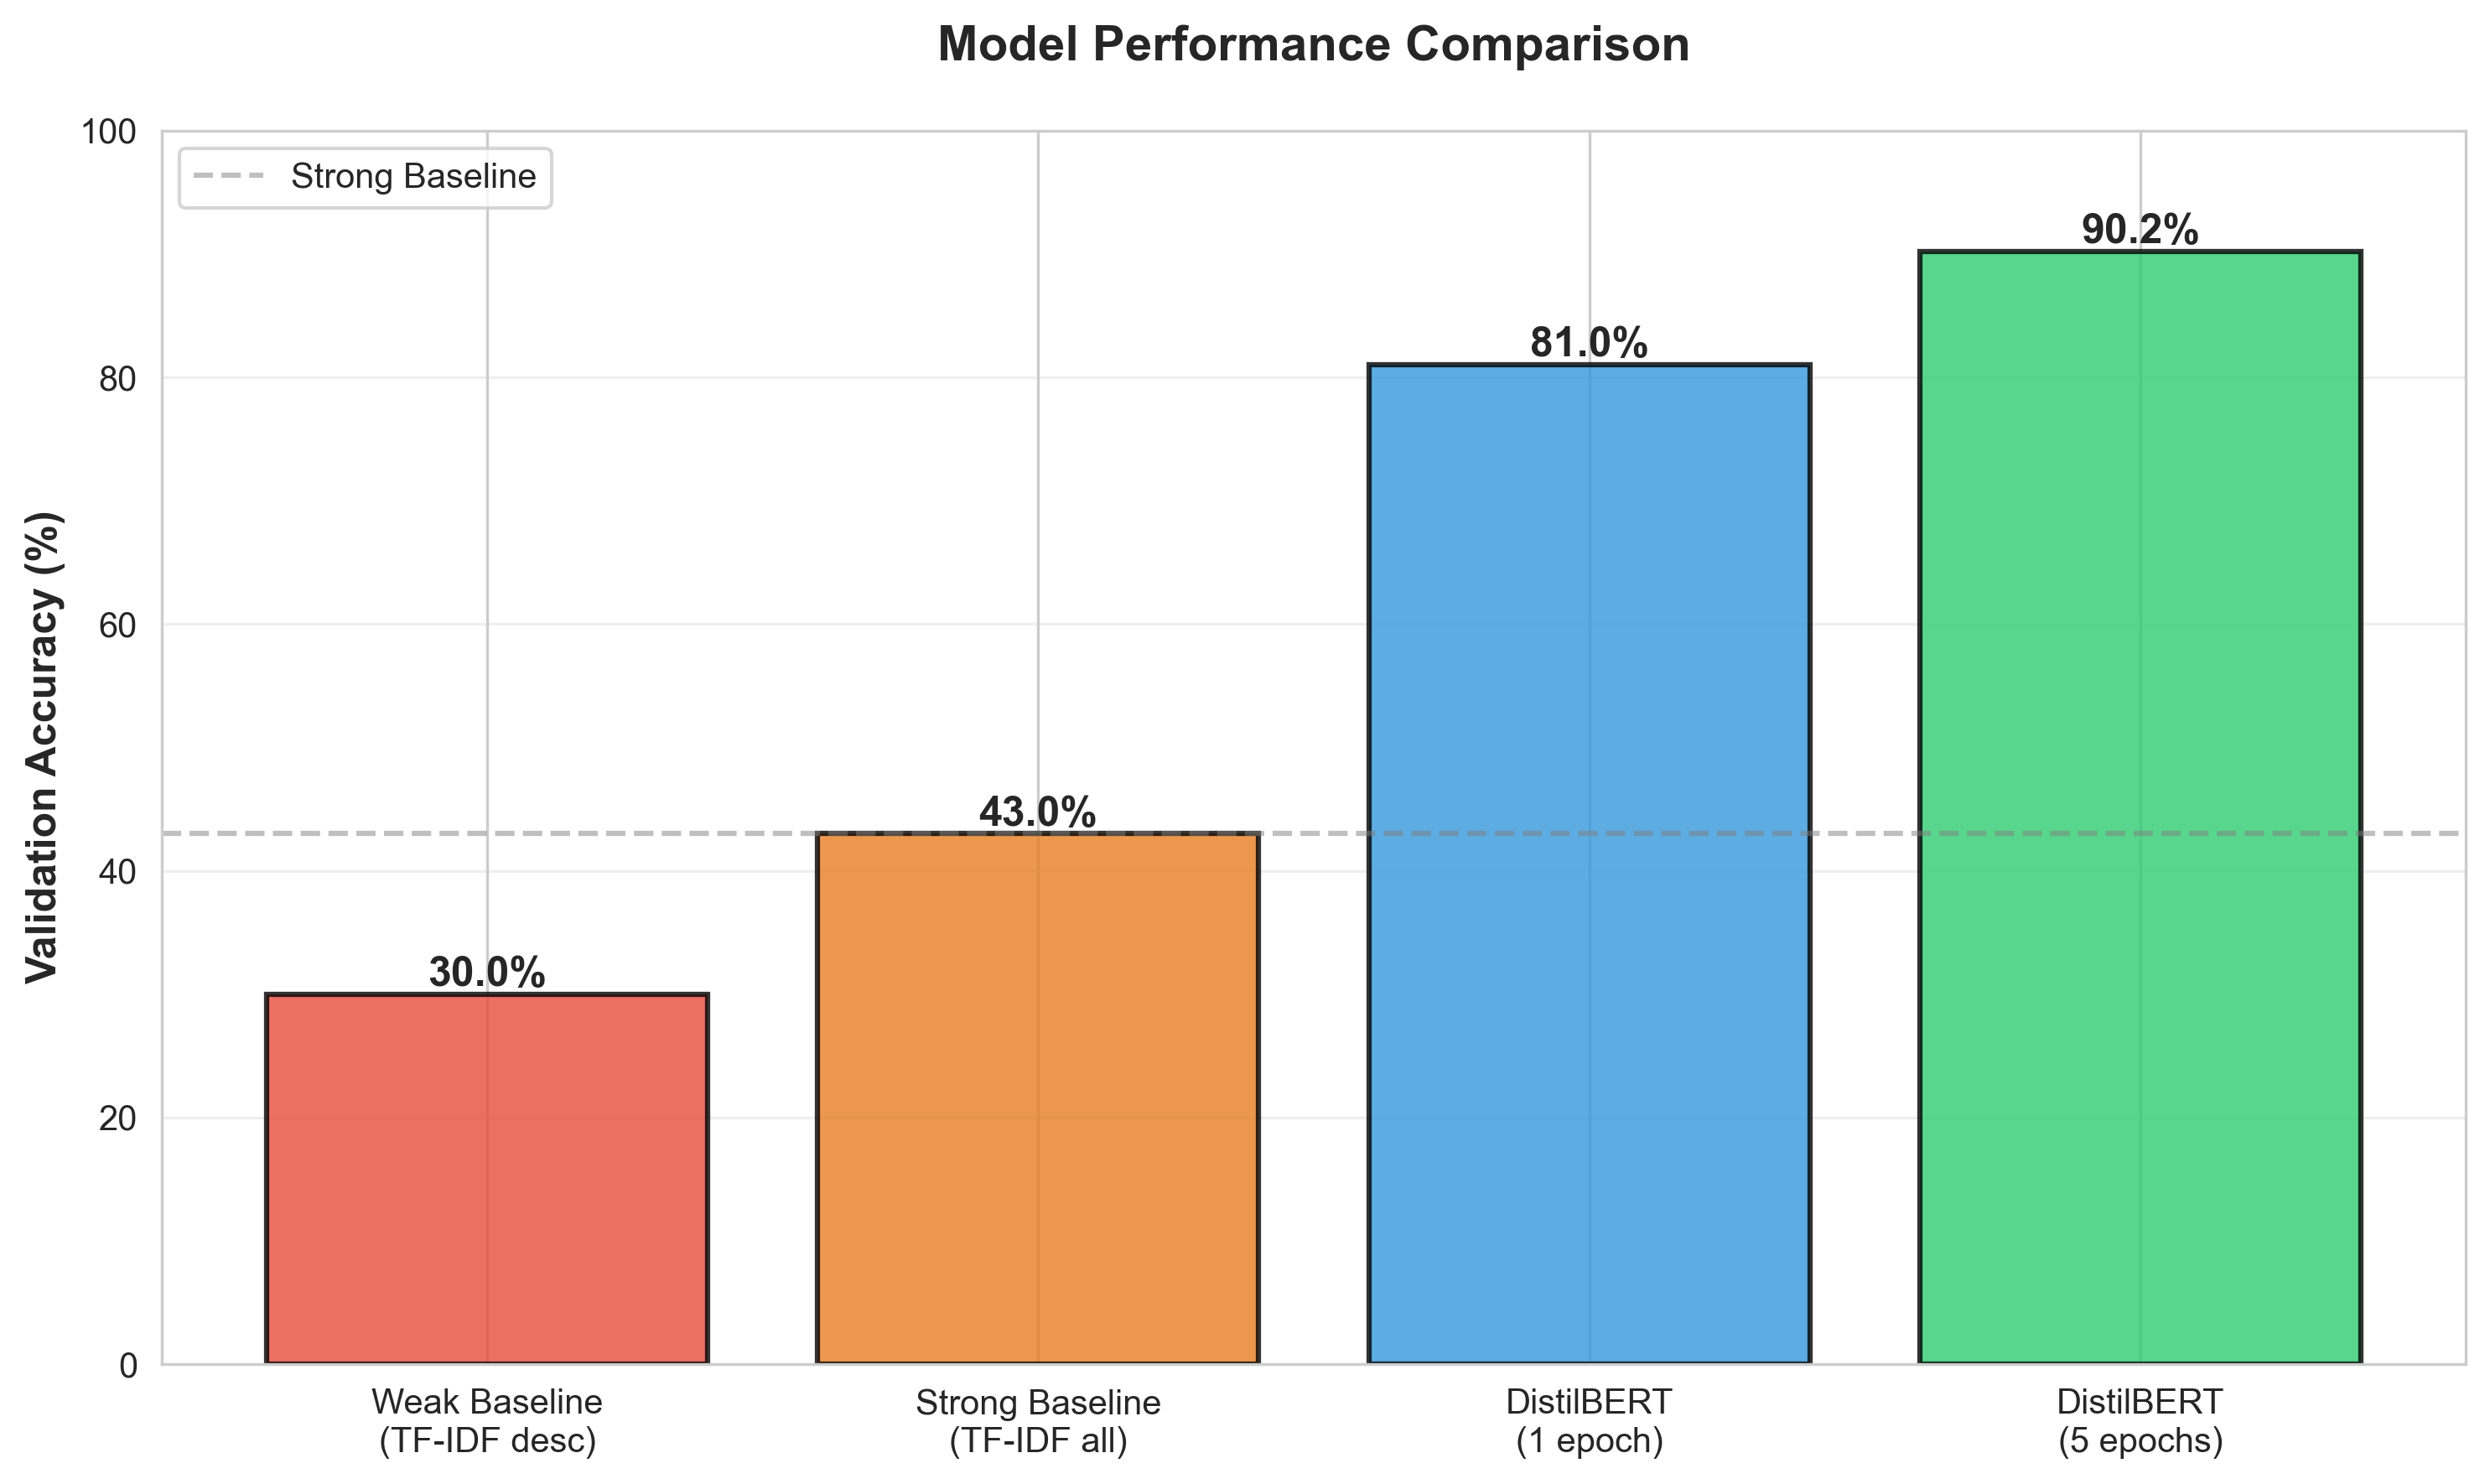
\includegraphics[width=0.85\textwidth]{../results/figures/baseline_comparison.png}
\end{center}
\end{frame}

% Slide 5: Training Curves
\begin{frame}{Training Progress}
\begin{center}
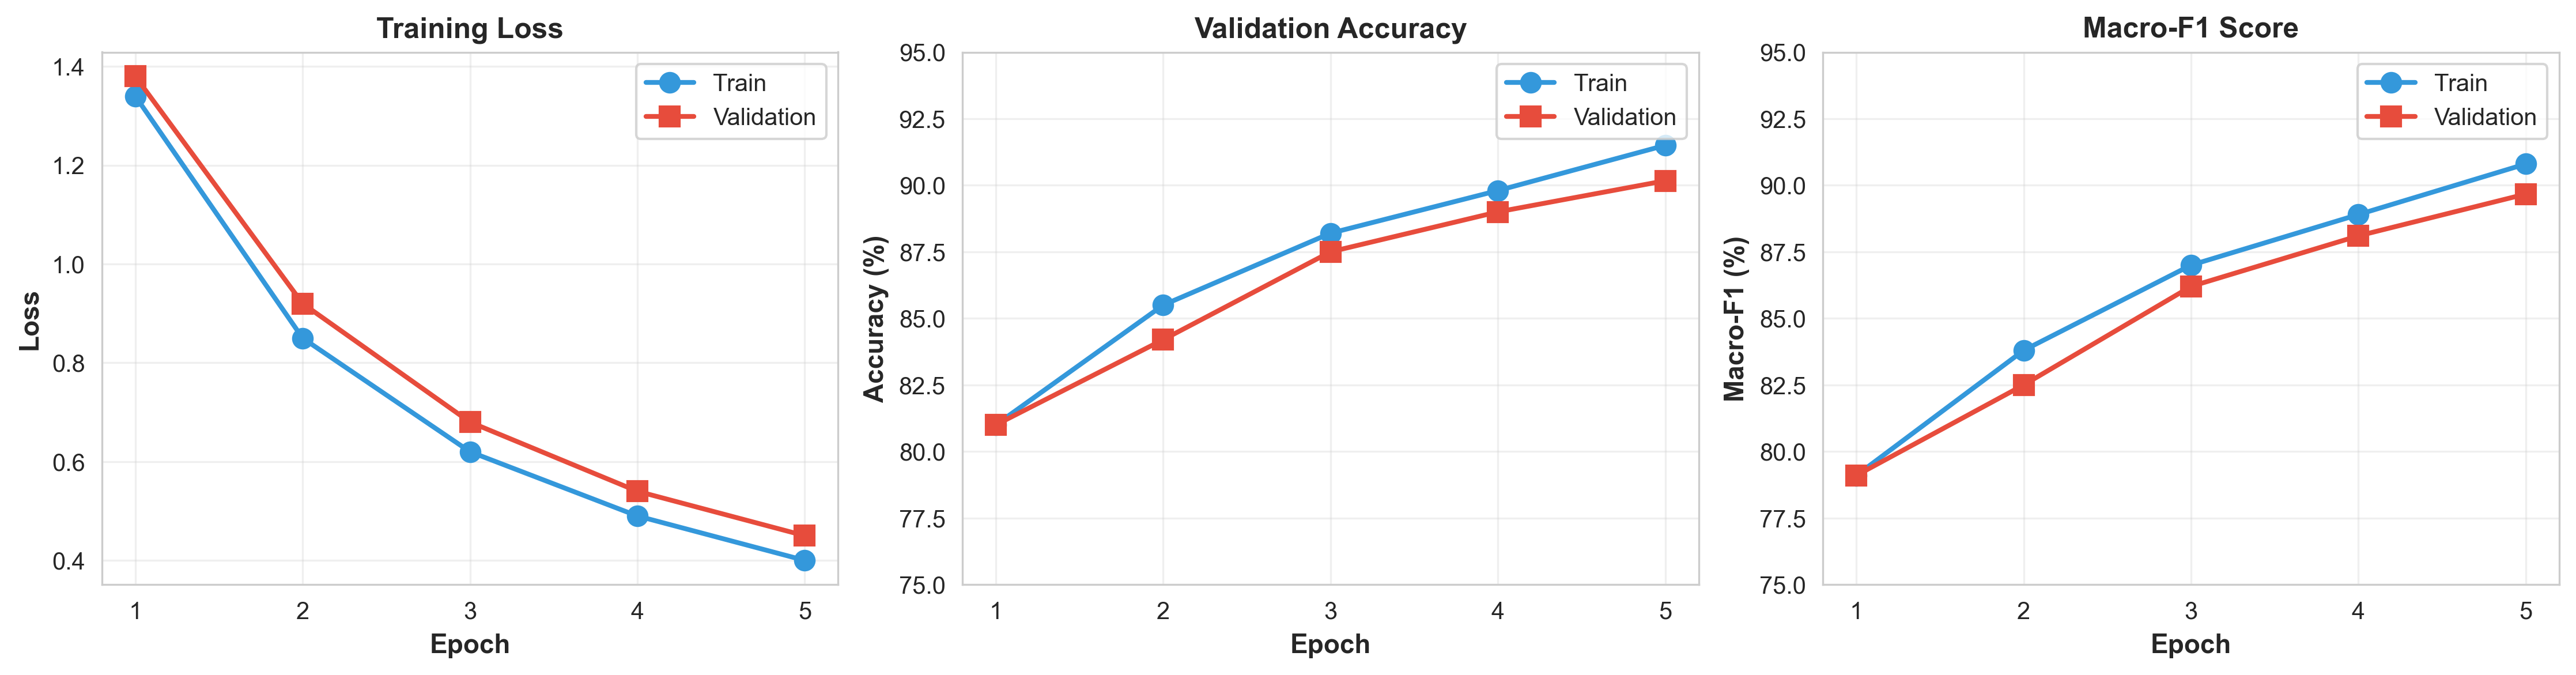
\includegraphics[width=\textwidth]{../results/figures/training_curves.png}
\end{center}
Steady improvement across 5 epochs, no overfitting
\end{frame}

% Slide 6: Distribution Comparison
\begin{frame}{Predictions Match Training Distribution}
\begin{center}
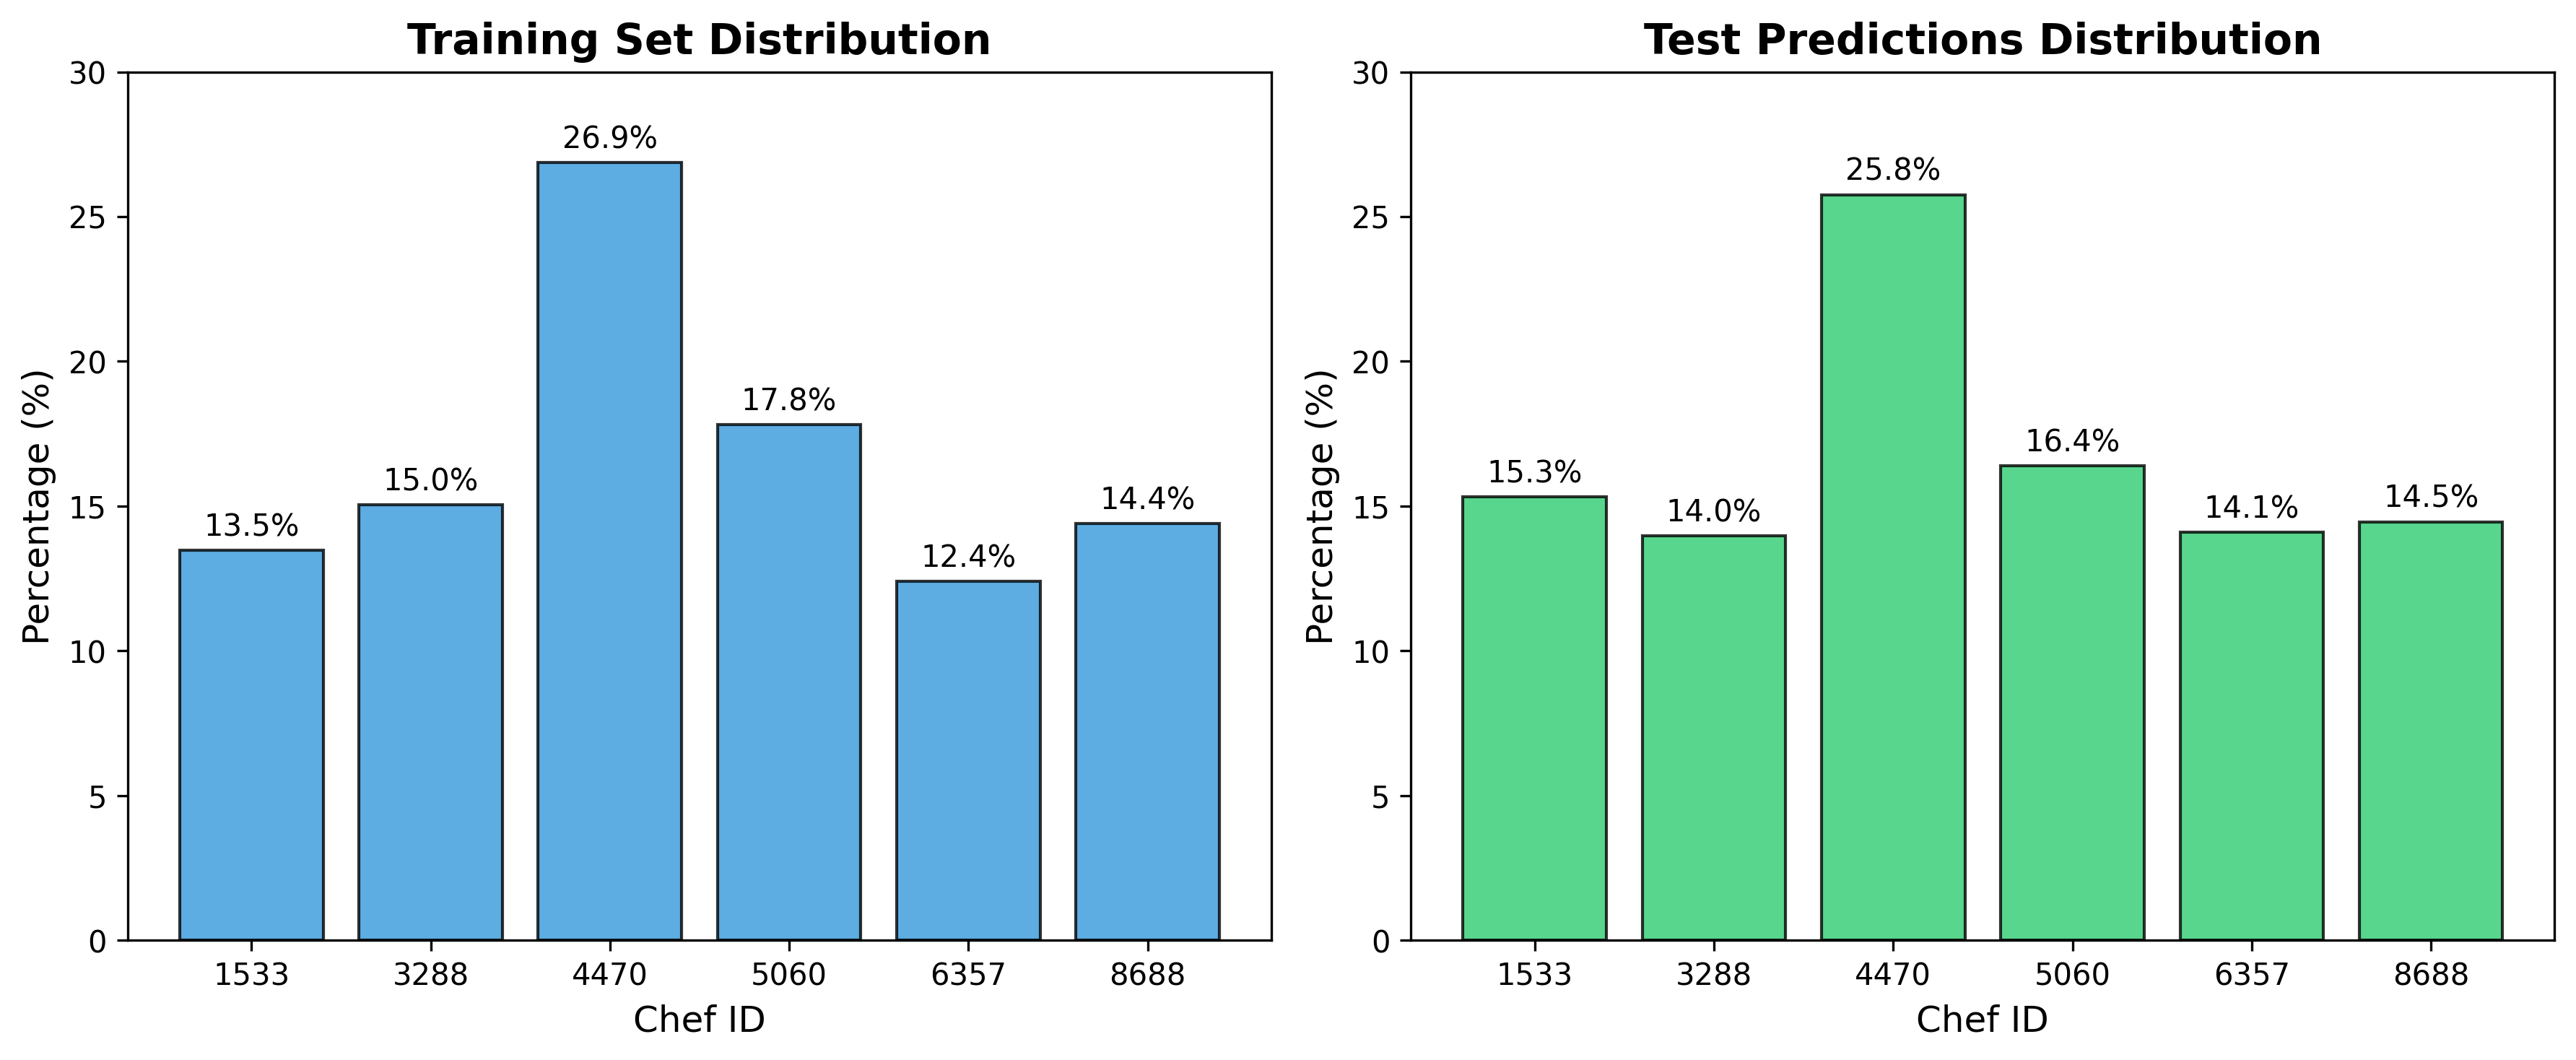
\includegraphics[width=\textwidth]{../results/figures/distribution_comparison.png}
\end{center}
\small Model learned chef patterns, not just class frequencies! (All differences $<$ 2\%)
\end{frame}

% Slide 7: What Did Model Learn
\begin{frame}{What Did the Model Learn?}
\textbf{Chef signatures identified}:

\begin{enumerate}
    \item \textbf{Health-focused chef} (5060): ``diabetic cooking'', ``low-fat''
    \begin{itemize}
        \item Across recipes: fish, potatoes, pancakes
    \end{itemize}
    
    \item \textbf{Make-ahead chef} (3288): ``OAMC'', batch recipes
    \begin{itemize}
        \item ``freeze for future use'', family-friendly
    \end{itemize}
    
    \item \textbf{Quick \& simple chef} (6357): ``15-minutes-or-less''
    
    \item \textbf{Southern/traditional chef} (8688): Bread machine, Creole
\end{enumerate}

\vspace{0.3cm}
\textbf{Key insight}: Model distinguishes \emph{how} chefs cook, not just \emph{what}!
\end{frame}

% Slide 8: Challenges
\begin{frame}{Challenges \& Solutions}
\textbf{Challenge 1}: Mac overheating during training
\begin{itemize}
    \item \textbf{Solution}: ``Chill mode'' config
    \item Reduced batch size (16 $\rightarrow$ 8), lower GPU usage
    \item Same results, $\sim$25 min training time
\end{itemize}

\vspace{0.5cm}

\textbf{Challenge 2}: Class imbalance (2.17x)
\begin{itemize}
    \item \textbf{Solution}: Stratified splitting + macro-F1 metric
    \item Macro-F1 (89.67\%) $\approx$ Accuracy (90.17\%) $\rightarrow$ balanced!
\end{itemize}
\end{frame}

% Slide 9: Discussion
\begin{frame}{Discussion}
\textbf{Strengths}:
\begin{itemize}
    \item Dramatic improvement over baselines (+47 pp)
    \item Learns chef-specific patterns (not just topics)
    \item Robust generalization (dist. matches training)
\end{itemize}

\vspace{0.3cm}

\textbf{Limitations}:
\begin{itemize}
    \item Strong textual signals (``diabetic cooking'', ``OAMC'')
    \item Some recipes may be easy to classify
    \item Single model (no ensemble)
    \item Can't generalize to new chefs
\end{itemize}

\vspace{0.3cm}

\textbf{Critical question}: Style vs. topic?
\begin{itemize}
    \item Evidence for both (patterns + keywords)
    \item High accuracy might indicate topical clustering
\end{itemize}
\end{frame}

% Slide 10: Summary
\begin{frame}{Summary}
\begin{itemize}
    \item \textbf{90.17\% accuracy} (beat baseline by 47 pp)
    \item Learned chef signatures: health-focus, make-ahead, quick, traditional
    \item Practical solutions: thermal management, class imbalance
    \item Critical analysis: acknowledged limitations
\end{itemize}

\vspace{1cm}

\textbf{Key insight}: Look at predictions, not just metrics! \\
Model captures cooking philosophy across recipe types.
\end{frame}

% Slide 11: Questions
\begin{frame}
\begin{center}
{\Huge Questions?}

\vspace{1cm}

{\large Code \& Results:} \\
\texttt{github.com/nbirchde/NLP\_group2}

\vspace{0.5cm}

Thank you!
\end{center}
\end{frame}

\end{document}
